\documentclass{boi2014-lt}

\usepackage{enumitem}

\renewcommand{\DayNum}{2}
\renewcommand{\TaskCode}{postmen}
\renewcommand{\TaskName}{Senjorai paštininkai}

\begin{document}
    \begin{wrapfigure}[8]{r}{4cm}
        \vspace{-18pt}
		\includegraphics[width=4cm]{\TaskCode.jpeg}
	\end{wrapfigure}
	Dabar 2036-ieji metai ir Europa yra perpildyta garbaus amžiaus piliečiais.
	Tam, kad jie išsaugotų sveikatą, Europos daugumų ministerija (garbaus amžiaus
	piliečiai \emph{yra} dauguma!) siūlo įdarbinti juos popierinių laiškų,
	kurie vis dar yra siunčiama (dažniausiai būtent garbaus amžiaus piliečiams),
	išnešiotojais. Šis pasiūlymas bus realizuotas visoje Europoje, netgi
	nepriklausomose Norvegijos ir Šveicarijos valstijose.

    Ministerija sukūrė ``garbaus amžiaus piliečių sistemą'' padalindama visą
    Europą į pašto rajonus. Pašto rajoną -- tai gatvių tinklas, sudarytą iš
    gatvių ir sankryžų. Kiekviena gatve šiame tinkle galima eiti abejomis
    kryptimis. Kiekviename rajone paštininkais galima pasamdyti neribotą skaičių
    garbaus amžiaus piliečių. Kiekvieną rytą, kiekvienas paštininkas gauna krepšį
    su laiškais, kuriuos reikia pristatyti keliaujant maršrutu, dengiančiu dalį
    gatvių tinklo. Kiekvienas maršrutas turi būti tinkamas garbiam amžiui, t.~y.
    jis turi tenkinti šias sąlygas:
	\todo{graph theory terminology here?}
    \begin{itemize}
        \item Prasidėti ir baigtis toje pačioje sankryžoje. (Hey, it’s a tour!)
        \item Nekirsti jokios sankryžos daugiau nei vieną kartą. (Nepainiokite
            garbaus amžiaus piliečių.)
        \item Neturėti bendrų gatvių su kitais maršrutais, t.~y. kiekvieną gatvę
            aptarnauja lygiai vienas paštininkas. (Garbaus amžiaus piliečiai
            neturėtų peštis tarpusavyje.)
    \end{itemize}

    Visi maršrutai kartu privalo pilnai padengti duotą gatvių tinklą: t.~y.
    kiekviena tinklo gatvė turi būti lygiai vieno maršruto dalimi.

    \Task
    Ministerija prašo jūsų sukurti programą, kuri duotam pašto rajono gatvių
    tinklui surastų garbiam amžiui tinkamų maršrutų aibę, kuri pilnai padengtų
    gatvių tinklą.

    \Input
    Įvestis apibūdina gatvių tinklą.
    
    Pirmoje eilutėje yra du sveikieji skaičiai $N$ ir $M$. $N$ -- sankryžų gatvių
    tinkle skaičius, $M$ -- gatvių tinkle skaičius. Sankryžos numeruojamos nuo
    $1$ iki $N$.

    Toliau kiekvienoje iš $M$ eilučių yra du sveikieji skaičiai $U$ ir $V$, reiškiantys, kad šios gatvių sankryžos yra sujungtos gatve.
    %\todo{missing $V$ in english task}

    For any input holds:
    \begin{enumerate}
        \item For any two junctions, you can walk from one junction to the other.
        \item There is a solution, i.e. a set of senior-compatible tours can be
        computed that cover the network.
    \end{enumerate}

    \Output
    The first output line is to contain an integer $T$, the number of tours.

    The $T$ tours are described in the following $T$ lines. Each of these lines
    is to contain at first the number $C$ of different junctions the mailman has
    to pass on this tour. The following $C$ integers in the line are the numbers
    of the junctions in this tour. They must be output in the order the
    junctions are passed by the mailman, with the starting (and ending) junction
    being output first (and only once).

    If there are two or more solutions, your program may output any of them.

    \Example

    \example
    {
        10 15 \newline
        1 2 \newline
        5 1\newline
        2 3 \newline
        9 2\newline
        3 4 \newline
        6 3\newline
        4 5 \newline
        7 4\newline
        4 8 \newline
        5 7 \newline
        8 5\newline
        6 7 \newline
        7 8 \newline
        8 10 \newline
        10 9
    }
    {
        3 \newline
        7 2 3 4 5 8 10 9 \newline
        3 4 7 8 \newline
        5 1 5 7 6 3
    }
    {
        The following picture illustrates the street network and the three
        senior-compatible tours that may be used to cover it.

        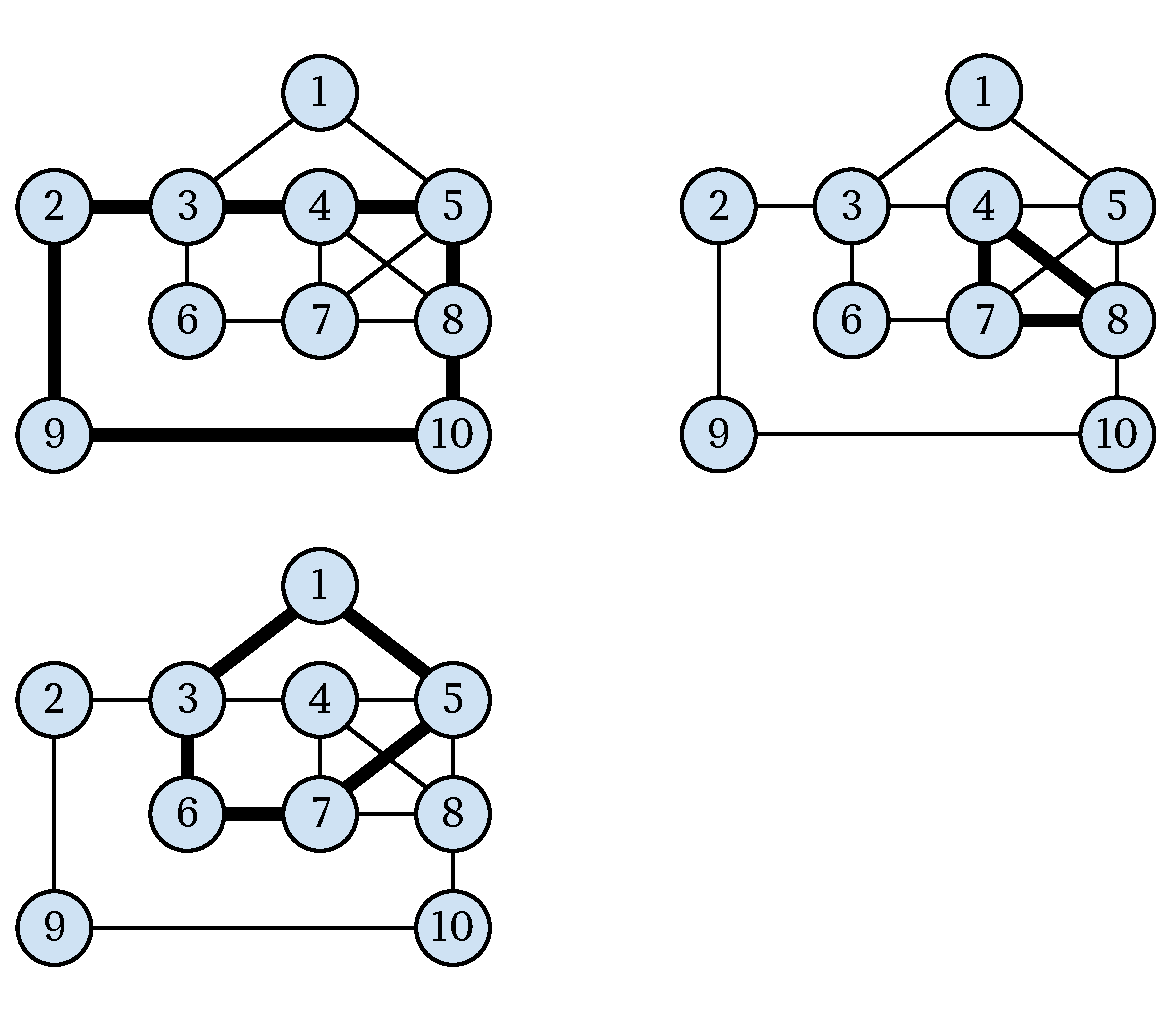
\includegraphics[width=7cm]{senior-example}

        Note that there are several solutions to this example, among them some
        with only two tours.
    
    }

    \Scoring

    \begin{description}
        \item[Subtask 1 (40 points):] $1 \le N \le 2\ 000$, $1 \le M \le 100\ 000$.
        \item[Subtask 2 (20 points):] $1 \le N \le 100\ 000$, $1 \le M \le 100\ 000$.
        \item[Subtask 3 (40 points):] $1 \le N \le 500\ 000$, $1 \le M \le 500\ 000$.
    \end{description}

    \Constraints

    \begin{description}
        \item[Time limit:] 1 s.
        \item[Memory limit:] 256 MB.
    \end{description}

\end{document}
